              %******************************************%
              %                                          %
              % Modello di tesi di laurea o di dottorato %
              %            di Lorenzo Pantieri           %
              %                                          %
              %                © 2013-2017               %
              %                                          %
              %******************************************%
       

% I seguenti commenti speciali impostano:
% 1. utf8 come codifica di input,
% 2. PDFLaTeX come motore di composizione;
% 3. Tesi.tex come documento principale;
% 4. il controllo ortografico italiano per l'editor.

% !TEX encoding = UTF-8 Unicode
% !TEX TS-program = pdflatex
% !TEX root = Tesi.tex
% !TEX spellcheck = it-IT

\documentclass[11pt,%                      % corpo del font principale
               a4paper,%                   % carta A4
%              twoside,openright,%         % fronte-retro
               oneside,openany,%           % solo fronte
               titlepage,%                 % frontespizio
               headinclude,,footinclude,%  % testatina e piede di pagina
               BCOR5mm,%                   % rilegatura di 5 mm
               cleardoublepage=empty,%     % pagine vuote senza testatina e piede di pagina
               captions=tableheading,%     % didascalie in cima alle tabelle
               ]{scrreprt}                 % classe report di KOMA-Script;
               
\usepackage[T1]{fontenc}                   % codifica dei font:
                                           % NOTA BENE! richiede una distribuzione *completa* di LaTeX,
                                           % per esempio TeXLive o MiKTeX *complete*

\usepackage[utf8]{inputenc}                % codifica di input; anche [latin1] va bene
                                           % NOTA BENE! va accordata con le preferenze dell'editor

\usepackage[english,italian]{babel}        % per scrivere in italiano e in inglese;
                                           % l'ultima lingua (l'italiano) risulta predefinita

\usepackage[suftesi]{frontespizio}         % frontespizo
                                           % per includerlo nel documento bisogna:
                                           % 1. compilare una prima volta Tesi.tex;
                                           % 2. compilare a parte Tesi-frn.tex, generato dalla compilazione precedente;
                                           % 3. compilare ancora Tesi.tex. 

%\usepackage{indentfirst}                   % rientra il primo capoverso di ogni sezione

\usepackage{graphicx}                      % immagini

\usepackage{listings}                      % codici

\usepackage[font=small]{quoting}           % citazioni

\usepackage{amsmath,amssymb,amsthm}        % matematica

\usepackage[italian]{varioref}             % riferimenti completi della pagina

\usepackage{tabularx}                      % tabelle di larghezza prefissata

\usepackage[autostyle,italian=guillemets]{csquotes} % virgolette ottimizzate per biblatex

\usepackage[style=philosophy-modern,hyperref,square,backend=biber]{biblatex}
                                           % eccellente pacchetto per la bibliografia;
                                           % produce uno stile di citazione autore-anno; 
                                           % lo stile "numeric-comp" produce riferimenti numerici;
                                           % NOTA BENE! bisogna che il proprio editor sia configurato per biber
                                          
\addbibresource{Bibliografia.bib}          % database di biblatex 
                                          
\usepackage{subfig}                        % sottofigure, sottotabelle

\usepackage{lipsum}                        % testo fittizio

\usepackage{eurosym}                       % simbolo dell'euro

\usepackage[eulerchapternumbers,%          % numeri dei capitoli nel font Euler
            subfig,%                       % se si usa il pacchetto subfig
            beramono,%                     % Bera Mono come font a spaziatura fissa
            eulermath,%                    % AMS Euler come font per la matematica
            pdfspacing,%                   % migliora il riempimento di riga
            listings,%                     % codici
%           parts,%                        % da decommentare in un documento diviso in parti
            ]{classicthesis}               % stile ClassicThesis

\usepackage{arsclassica}                   % modifica l'aspetto di ClassicThesis

%*********************************************************************************
% impostazioni-tesi.tex
% di Lorenzo Pantieri (2013-2016)
% file che contiene le impostazioni della tesi
%*********************************************************************************


%*********************************************************************************
% Comandi personali
%*******************************************************
\newcommand{\myName}{Michele Vaccari}                            % autore
\newcommand{\myTitle}{Progetto E-Commerce BINS}                  % titolo
\newcommand{\myDegree}{Documentazione Ingegneria del Software}   % tipo di tesi
\newcommand{\myUni}{Universit\'a degli Studi di Ferrara}         % universit�
\newcommand{\myFaculty}{Facolt\'a di Ingegneria}                 % facolt\'a
\newcommand{\myDepartment}{Dipartimento di Ingegneria}           % dipartimento
\newcommand{\myProf}{Prof.~Fabrizio~Luglio}                      % relatore
%\newcommand{\myOtherProf}{Dott.~Immanuel Kant}                  % correlatore (se presente)
\newcommand{\myLocation}{Castagnaro}                             % dove
\newcommand{\myTime}{Settembre 2017}                             % quando



%*********************************************************************************
% Impostazioni di amsmath, amssymb, amsthm
%*********************************************************************************

% comandi per gli insiemi numerici (serve il pacchetto amssymb)
\newcommand{\numberset}{\mathbb} 
\newcommand{\N}{\numberset{N}} 
\newcommand{\R}{\numberset{R}} 

% un ambiente per i sistemi
\newenvironment{sistema}%
  {\left\lbrace\begin{array}{@{}l@{}}}%
  {\end{array}\right.}

% definizioni (serve il pacchetto amsthm)
\theoremstyle{definition} 
\newtheorem{definizione}{Definizione}

% teoremi, leggi e decreti (serve il pacchetto amsthm)
\theoremstyle{plain} 
\newtheorem{teorema}{Teorema}
\newtheorem{legge}{Legge}
\newtheorem{decreto}[legge]{Decreto}
\newtheorem{murphy}{Murphy}[section]



%*********************************************************************************
% Impostazioni di biblatex
%*********************************************************************************
\defbibheading{bibliography}{%
\cleardoublepage
\manualmark
\phantomsection 
\addcontentsline{toc}{chapter}{\tocEntry{\bibname}}
\chapter*{\bibname\markboth{\spacedlowsmallcaps{\bibname}}
{\spacedlowsmallcaps{\bibname}}}}



%*********************************************************************************
% Impostazioni di listings
%*********************************************************************************
\lstset{language=[LaTeX]Tex,%C++,
    keywordstyle=\color{RoyalBlue},%\bfseries,
    basicstyle=\small\ttfamily,
    %identifierstyle=\color{NavyBlue},
    commentstyle=\color{Green}\ttfamily,
    stringstyle=\rmfamily,
    numbers=none,%left,%
    numberstyle=\scriptsize,%\tiny
    stepnumber=5,
    numbersep=8pt,
    showstringspaces=false,
    breaklines=true,
    frameround=ftff,
    frame=single
} 



%*********************************************************************************
% Impostazioni di hyperref (decommenta le seguenti righe se non carichi arsclassica)
%*********************************************************************************
%\hypersetup{%
%    hyperfootnotes=false,pdfpagelabels,
%    %draft,	% = elimina tutti i link (utile per stampe in bianco e nero)
%    colorlinks=true, linktocpage=true, pdfstartpage=1, pdfstartview=FitV,%
%    % decommenta la riga seguente per avere link in nero (per esempio per la stampa in bianco e nero)
%    %colorlinks=false, linktocpage=false, pdfborder={0 0 0}, pdfstartpage=1, pdfstartview=FitV,% 
%    breaklinks=true, pdfpagemode=UseNone, pageanchor=true, pdfpagemode=UseOutlines,%
%    plainpages=false, bookmarksnumbered, bookmarksopen=true, bookmarksopenlevel=1,%
%    hypertexnames=true, pdfhighlight=/O,%nesting=true,%frenchlinks,%
%    urlcolor=webbrown, linkcolor=RoyalBlue, citecolor=webgreen, %pagecolor=RoyalBlue,%
%    %urlcolor=Black, linkcolor=Black, citecolor=Black, %pagecolor=Black,%
%    pdftitle={\myTitle},%
%    pdfauthor={\textcopyright\ \myName, \myUni, \myFaculty},%
%    pdfsubject={},%
%    pdfkeywords={},%
%    pdfcreator={pdfLaTeX},%
%    pdfproducer={LaTeX with hyperref and ClassicThesis}%
%}



%*********************************************************************************
% Impostazioni di graphicx
%*********************************************************************************
\graphicspath{{immagini/}} % cartella dove sono riposte le immagini



%*********************************************************************************
% Margini ottimizzati per l'A4
%*********************************************************************************
\areaset[current]{370pt}{750pt}
\setlength{\marginparwidth}{7em}
\setlength{\marginparsep}{2em}%



%*********************************************************************************
% Impostazioni di varioref
%*********************************************************************************
\makeatletter
\vref@addto\extrasitalian{%
   \def\reftextfaraway#1{a pagina~\pageref{#1}}%
}
\makeatother



%*********************************************************************************
% Altro
%*********************************************************************************

% [...] ;-)
\newcommand{\omissis}{[\dots\negthinspace]}

% eccezioni all'algoritmo di sillabazione
\hyphenation{Fortran ma-cro-istru-zio-ne nitro-idrossil-amminico}

% correzione di un bug di scrreprt nella numerazione delle figure
\renewcommand*{\figureformat}{%
  \figurename~\thefigure%
  %\autodot%
}
\renewcommand*{\tableformat}{%
  \tablename~\thetable%
  %\autodot%
}                  % file con le impostazioni personali


\begin{document}
\pagestyle{scrheadings} 
\pagenumbering{roman}
%******************************************************************
% Materiale iniziale
%******************************************************************
% !TEX encoding = UTF-8
% !TEX TS-program = pdflatex
% !TEX root = ../Tesi.tex
% !TEX spellcheck = it-IT

%*******************************************************
% Frontespizio
%*******************************************************
\begin{frontespizio}
\Preambolo{\usepackage{iwona}} % riga da commentare se non si carica ArsClassica

\Universita{Ferrara}
\Logo{logo-unife}
%\Facolta{Ingegneria}
\Dipartimento{Ingegneria}
\Corso[Laurea Triennale]{Ingegneria Elettronica e Informatica}
\Annoaccademico{2016--2017}
\Titoletto{Documentazione Basi di Dati}
\Titolo{Progetto E-Commerce: \\ BINS}
%\Sottotitolo{Alcune considerazioni mutevoli}
\NCandidato{Studente}
\Candidato[121955]{Michele Vaccari}
\NRelatore{Docente}{}
\Relatore{Prof. Denis Ferraretti}
%\Relatore{Claudio Beccari}
%\Correlatore{Tommaso Gordini}
%\Correlatore{Ivan Valbusa}
\end{frontespizio}
% !TEX encoding = UTF-8
% !TEX TS-program = pdflatex
% !TEX root = ../Tesi.tex
% !TEX spellcheck = it-IT

%*******************************************************
% Colophon
%*******************************************************
\clearpage
\phantomsection
\thispagestyle{empty}

\hfill

\vfill

\noindent\myName: \textit{\myTitle,}
\myDegree,
\textcopyright\ \MakeTextLowercase{\myTime}.

%\lipsum[2]
%% !TEX encoding = UTF-8
% !TEX TS-program = pdflatex
% !TEX root = ../Tesi.tex
% !TEX spellcheck = it-IT

%*******************************************************
% Dedica
%*******************************************************
\cleardoublepage
\phantomsection
\thispagestyle{empty}
\pdfbookmark{Dedica}{Dedica}

\vspace*{3cm}

\begin{center}
Lorem ipsum dolor sit amet, consectetuer adipiscing elit. \\ \medskip
--- Oscar Wilde    
\end{center}

\medskip

\begin{center}
Dedicato a tutti gli appassionati di \LaTeX.
\end{center}
% !TEX encoding = UTF-8
% !TEX TS-program = pdflatex
% !TEX root = ../Tesi.tex
% !TEX spellcheck = it-IT

%*******************************************************
% Indici
%*******************************************************
\cleardoublepage
\pdfbookmark{\contentsname}{tableofcontents}
\setcounter{tocdepth}{2}
\tableofcontents
\markboth{\spacedlowsmallcaps{\contentsname}}{\spacedlowsmallcaps{\contentsname}} 
\clearpage

\begingroup 
    \let\clearpage\relax
    \let\cleardoublepage\relax
    %*******************************************************
    % Elenco delle figure
    %*******************************************************    
    \phantomsection
    \pdfbookmark{\listfigurename}{lof}
    \listoffigures

    \vspace*{8ex}

    %*******************************************************
    % Elenco delle tabelle
    %*******************************************************
    \phantomsection
    \pdfbookmark{\listtablename}{lot}
    %\listoftables
       
\endgroup

\cleardoublepage

%% !TEX encoding = UTF-8
% !TEX TS-program = pdflatex
% !TEX root = ../Tesi.tex
% !TEX spellcheck = it-IT

%*******************************************************
% Sommario+Abstract
%*******************************************************
\cleardoublepage
\phantomsection
\pdfbookmark{Sommario}{Sommario}
\begingroup
\let\clearpage\relax
\let\cleardoublepage\relax
\let\cleardoublepage\relax

\chapter*{Sommario}

\lipsum[1]

\vfill

\selectlanguage{english}
\pdfbookmark{Abstract}{Abstract}
\chapter*{Abstract}

\lipsum[2]

\selectlanguage{italian}

\endgroup			

\vfill


%% !TEX encoding = UTF-8
% !TEX TS-program = pdflatex
% !TEX root = ../Tesi.tex
% !TEX spellcheck = it-IT

%*******************************************************
% Ringraziamenti
%*******************************************************
\cleardoublepage
\phantomsection
\pdfbookmark{Ringraziamenti}{ringraziamenti}

\chapter*{Ringraziamenti}

\begin{flushright}{\slshape    
	Lorem ipsum dolor sit amet, consectetuer adipiscing elit. \\
	Ut purus elit, vestibulum ut, placerat ac, adipiscing vitae, felis. \\
	Curabitur dictum gravida mauris.} \\ \medskip
    --- Donald Ervin Knuth
\end{flushright}

\lipsum[1]

\bigskip
 
\noindent\textit{\myLocation, \MakeTextLowercase{\myTime}}
% !TEX encoding = UTF-8
% !TEX TS-program = pdflatex
% !TEX root = ../Tesi.tex
% !TEX spellcheck = it-IT

%*******************************************************
% Introduzione
%*******************************************************
\cleardoublepage
\pdfbookmark{Introduzione}{introduzione}

\chapter*{Introduzione}

BINS (acronimo ricorsivo di "BINS Is Not Shopping") è un applicazione web liberamente disponibile, indicata soprattutto per commercializzare prodotti alimentari. Lo scopo di questo lavoro è di documentare l'applicazione usando l'UML (Unified Model Language).

La documentazione è articolata come segue.

\begin{description}
	\item[{\hyperref[cap:specifiche-progetto]{Il primo capitolo}}]
	contiene le specifiche del progetto descrivendo le caratteristiche e le categorie di utenti dell'applicazione.
	\item[{\hyperref[cap:modello-casi-d'uso]{Il secondo capitolo}}]
	descrive che cosa deve fare il sistema e quali sono gli attori per poterlo far funzionare.
	\item[{\hyperref[cap:modello-del-dominio]{Il terzo capitolo}}]
	descrive quali sono le informazioni che il sistema deve trattare e quali non deve trattare.
	\item[{\hyperref[cap:modello-di-design]{Il quarto capitolo}}]
	descrive nel dettaglio la struttura fisica dell'applicazione.
\end{description}

Per il \emph{Presentation Level} si è usato il framework \emph{Bootstrap} sfruttando al meglio il \emph{responsive design} che viene messo a disposizione dal framework. Per quanto riguarda l'usabilità e il design si è scelto l'approccio \emph{mobile first} ma si è anche prestato attenzione all'uso dell'applicazione in modalità desktop.

Per l'application server si è usato \emph{Tomcat} e si è utilizzato il linguaggio di progammazione Java.
 Per interfacciare l'application server con il database si è utilizzato JDBC.
 
Il DBMS utilizzato è \emph{MySQL}.

Di seguito si riporta il diagramma approssimato relativo allo sviluppo del lavoro in termini di tempo attraverso un diagramma di Gantt:
\cleardoublepage
%******************************************************************
% Materiale principale
%******************************************************************
\pagenumbering{arabic}
% !TEX encoding = UTF-8
% !TEX TS-program = pdflatex
% !TEX root = ../Tesi.tex
% !TEX spellcheck = it-IT

%************************************************
\chapter{Specifiche progetto}
\label{cap:specifiche-progetto}
%************************************************

\section{Caratteristiche del sistema}
Si vuole progettare un'applicazione web per la vendita on line dei prodotti di un supermercato.
L'applicazione deve avere un frontend multilingue (italiano e inglese).

I prodotti del supermercato sono suddivisi in reparti (ortofrutta, macelleria, accessori per la casa, cura della persona, ecc.) e ogni prodotto può avere una data di scadenza.

L'applicazione web deve avere le seguenti caratteristiche:

\begin{enumerate}
		
	\item
		\label{f-up}
		Possibilità di visualizzare il catalogo dei prodotti, navigabile per reparto, caratteristiche, marchio, ricerca libera, ecc.
		Possibilità di vedere il singolo prodotto con tutti i dettagli;
		
	\item
		Possibilità di inserire prodotti nel carrello e di effettuare l'acquisto di più prodotti in diverse quantità.
		Predisporre la gestione dei prezzi, del totale carrello, la gestione della disponibilità di magazzino, impedendo di poter acquistare quantità non disponibili e prodotti scaduti;
		
	\item
		Gestione di una o più shopping list (lista della spesa);
		
	\item
		Possibilità di inserire o selezionare un indirizzo di consegna da una rubrica personale, di simulare il pagamento e di confermare l'ordine;
		
	\item
		Possibilità di visualizzare lo stato dell'ordine e lo storico degli ordini effettuati;
		
	\item
		\label{ef-ur}
		Gestione di coupon o buoni sconto in fase di acquisto, possibilità di visualizzare il traking dell'ordine in consegna;
		
	\item
		\label{sf-ua}
		Possibilità di gestire il catalogo (inserimento, modifica, blocco prodotti), i reparti, i brand, ecc.
		Possibilità di gestire la disponibilità di magazzino;
	
	\item
		Gestione di prodotti in push (per cui spingere la vendita) con inserimento in una "vetrina in home page" o in un'area promo;
	
	\item
		Possibilità di visualizzare gli utenti, verificare il numero degli ordini per utente, bloccare eventuali utenti, gestire gli altri utenti amministratori;
	
	\item
		Gestione dei coupon o buoni sconto;
	
	\item
		\label{ef-ua}
		Gestione del tracking dell'ordine, con simulazione di tutti i cambi di stato (consegnato al corriere, in viaggio, consegnato al destinatario, ecc.);
		
\end{enumerate}

\section{Utenti del sistema}
Il sistema prevede che le categorie di utenti sia così rappresentata:

\begin{description}
	
	\item[Utenti pubblici] Possono effettuare solo il punto \ref{f-up} ed eventualmente registrarsi.
	
	\item[Utenti registrati] Possono effettuare i punti dal \ref{f-up} al \ref{ef-ur} compresi.
	
	\item[Amministratori] Possono effettuare i punti dal \ref{sf-ua} al \ref{ef-ua} compresi.
	
\end{description}   % specifiche del progetto
% !TEX encoding = UTF-8
% !TEX TS-program = pdflatex
% !TEX root = ../Tesi.tex
% !TEX spellcheck = it-IT

%************************************************
\chapter{Modello dei casi d'uso}
\label{cap:modello-casi-d'uso}
%************************************************

Si esegue l'analisi dei casi d'uso nel dominio degli attori che interessano i casi d'uso medesimi suddividendo lo schema completo in sottoschemi, uno per ogni attore, al fine di mantenere una maggior leggibilità del progetto. \\
Si documenta ogni caso d'uso al fine di descrivere nel dettaglio il comportamento del sistema senza riferirsi ad una particolare implementazione.

\section{Attore utente pubblico}
%
% Figura: casi d'uso dell'attore utente pubblico
%
\begin{figure}[h]
	\centering
	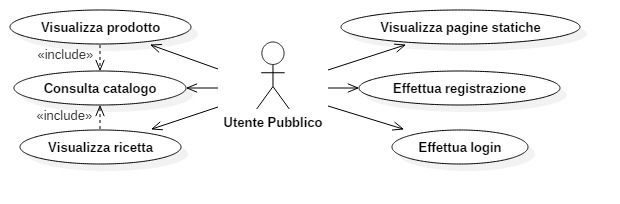
\includegraphics[width=1\textwidth]
	{immagini/attore-utente-pubblico}
	
	\caption{Casi d'uso dell'attore utente pubblico}
\end{figure}

%
% Caso d'uso: Consulta catalogo
%
\subsection{Caso d'uso: Consulta catalogo}

\subsubsection*{Descrizione}
Questa funzionalità permette all'utente pubblico di visualizzare il catalogo dei prodotti navigabile per reparto, caratteristiche, marchio e ricerca libera.

\subsubsection*{Attori coinvolti}
Utente pubblico, partecipazione attiva dell'attore verso il caso d'uso medesimo.

\subsubsection*{Pre-condizioni}
Nessuna precondizione.

\subsubsection*{Post-condizioni}
Nessuna postcondizione, in quanto la consultazione del catalogo non altera lo stato dell'applicazione.

\subsubsection*{Flusso principale}

\begin{enumerate}
	
	\item
	Il form per la ricerca libera e il menù per la consultazione del catalogo per reparti è visibile in tutte le pagine del sito;
	
	\item
	L'utente visualizza tutti i reparti;
	
	\item
	Il sistema visualizza all'utente tutti i reparti;
	
	\item
	L'utente seleziona un reparto;
	
	\item
	Il sistema visualizza all'utente tutti i prodotti dei prodotti che fanno parte del reparto selezionato;
	
	\item
	L'utente seleziona una o più caratteristiche e uno o più marchi per i prodotti di un reparto;
	
	\item
	Il sistema visualizza all'utente i risultati dei prodotti che soddisfano i criteri selezionati.
	
	\item
	L'utente pubblico inserisce del testo nel form per la ricerca libera;
	
	\item
	L'utente pubblico ha la possibilità di scegliere un reparto in cui effettuare una ricerca oppure estendere la ricerca a tutti i reparti;
	
	\item
	L'utente clicca sul pulsante per la ricerca e vengono inviati i dati al server;
	
	\item
	Il sistema effettua la ricerca del testo inserito dall'utente nei vari campi della tabella dei prodotti della base dati;
	
	\item
	Il sistema visualizza la tabella dei prodotti che soddisfano i campi della ricerca, ovvero fanno parte della tabella tutti i prodotti che contengono nei loro campi almeno una ricorrenza del testo da ricercare; 
	
	\item
	L'utente può raffinare la ricerca selezionando una o più caratteristiche e uno o più marchi per i prodotti di un reparto;
	
\end{enumerate}

\subsubsection*{Flussi alternativi}
Non presenti.

%
% Caso d'uso: Visualizza pagine statiche
%
\subsection{Caso d'uso: Visualizza pagine statiche}

	\subsubsection*{Descrizione}
	Questa funzionalità permette all'utente pubblico di visualizzare tutte le pagine richieste con contenuto non dinamico.
	
	\subsubsection*{Attori coinvolti}
	Utente pubblico, partecipazione attiva, richiedendo la visualizzazione delle pagine.
	
	\subsubsection*{Pre-condizioni}
	Nessuna precondizione, in quanto non serve uno stato particolare per visualizzare una pagina statica.
	
	\subsubsection*{Post-condizioni}
	Nessuna postcondizione, in quanto la visualizzazione di una pagina statica non altera lo stato dell'applicazione.
	
	\subsubsection*{Flusso principale}
	
	\begin{enumerate}
		
		\item
		Richiesta di qualsiasi pagina che abbia contenuto statico da parte dell'utente pubblico
		
		\item
		Risposta del server con la pagina statica richiesta da parte dell'utente pubblico;
		
	\end{enumerate}
	
	\subsubsection*{Flussi alternativi}
	Non presenti.

%
% Caso d'uso: Effettua registrazione
%
\subsection{Caso d'uso: Effettua registrazione}

	\subsubsection*{Descrizione}
	Questa funzionalità permette di registrare l'utente all'interno del database, consentendogli tutte le operazioni dell'utente registrato.
	
	\subsubsection*{Attori coinvolti}
	Utente pubblico, partecipazione attiva dell'attore verso il caso d'uso medesimo.
	
	\subsubsection*{Pre-condizioni}
	Nessuna precondizione.
	
	\subsubsection*{Post-condizioni}
	Viene aggiornato lo stato sul database con l'inserimento di un nuovo utente.
	
	\subsubsection*{Flusso principale}
	
		\begin{enumerate}
			
			\item
			L'utente visualizza il form da compilare per effettuare la registrazione nel sistema;
			
			\item
			L'utente compila tutti i campi visualizzati nel modulo con controllo diretto se i dati inseriti sono sintatticamente corretti oppure no;
			
			\item
			L'utente capisce che il dato inserito è sbagliato se il campo dove ha inserito l'informazione diventa di colore rosso, altrimenti se il colore è inalterato vuol dire che dal punto di vista sintattico le informazioni sono corrette;
			
			\item
			Finché il modulo non è stato inviato al server l'utente può modificare i dati inseriti negli appositi campi di compilazione;
			
			\item
			\label{fcu:effettua-registrazione}
			Quando l'utente richiede l'invio dei dati al server vengono controllati nuovamente tutti i campi del modulo, inoltre è richiesta l'accettazione delle condizioni di utilizzo;
			
			\item
			Una volta che i dati sono stati inviati al server vengono elaborati e memorizzati sul database modificando quindi lo stato del database stesso;
			
			\item
			Viene notificato all'utente l'avvenuto inserimento del proprio profilo nel sistema.
			
		\end{enumerate}
	
	\subsubsection*{Flussi alternativi}
	Nel caso di inserimento di un indirizzo email già esistente nel database, dopo il punto~\ref{fcu:effettua-registrazione} viene visualizzato nuovamente il form precompilato con i dati inseriti nell'ultima compilazione del form, notificando l'utente della presenza nel database di un profilo con lo stesso indirizzo email.

%
% Caso d'uso: Effettua login
%
\subsection{Caso d'uso: Effettua login}

	\subsubsection*{Descrizione}
	Questa funzionalità permette all'utente pubblico di farsi riconoscere dal sistema, accedendo quindi a tutte le sue funzionalità.
	
	\subsubsection*{Attori coinvolti}
	Utente pubblico, partecipazione attiva dell'attore che passa da \emph{Utente Pubblico} a \emph{Utente registrato} o \emph{Utente amministratore} o \emph{Utente super amministratore}.
	
	\subsubsection*{Pre-condizioni}
	Compilazione del modulo di login.
	
	\subsubsection*{Post-condizioni}
	L'utente passa da attore \emph{Utente Pubblico} ad attore \emph{Utente registrato} o ad attore \emph{Utente amministratore} o ad attore \emph{Utente super amministratore}.
	
	\subsubsection*{Flusso principale}
	
	\begin{enumerate}
		
		\item
		Il form per l'autenticazione è visibile in tutte le pagine del sito;
		
		\item
		L'utente pubblico compila il modulo inserendo la propria email e la propria password;
		
		\item
		Il sistema effettua verifica se le informazioni inserite nel campo email sono corrette dal punto di vista sintattico, colorando il campo di colore rosso se l'indirizzo inserito è sbagliato dal punto di vista sintattico;
		
		\item
		L'utente clicca sul pulsante per l'autenticazione e vengono inviati i dati al server;
		
		\item
		Dopo aver ricevuto i dati il server controlla se nella base dati è presente un utente con indirizzo email e password ricevuti;
		
		\item
		Se le informazioni esistono sulla base dati l'utente pubblico viene riconosciuto dal sistema e al posto del form per l'autenticazione viene visualizzato il nome dell'utente e un menù con tutte le operazioni che l'utente può eseguire sul sistema.
		
	\end{enumerate}
	
	\subsubsection*{Flussi alternativi}
	Nel caso di inserimento di email e password non presenti nel database vengono notificate all'utente pubblico le possibili cause di errore.

\section{Attore utente registrato}
%
% Figura: casi d'uso dell'attore utente registrato
%
\begin{figure}[h]
	\centering
	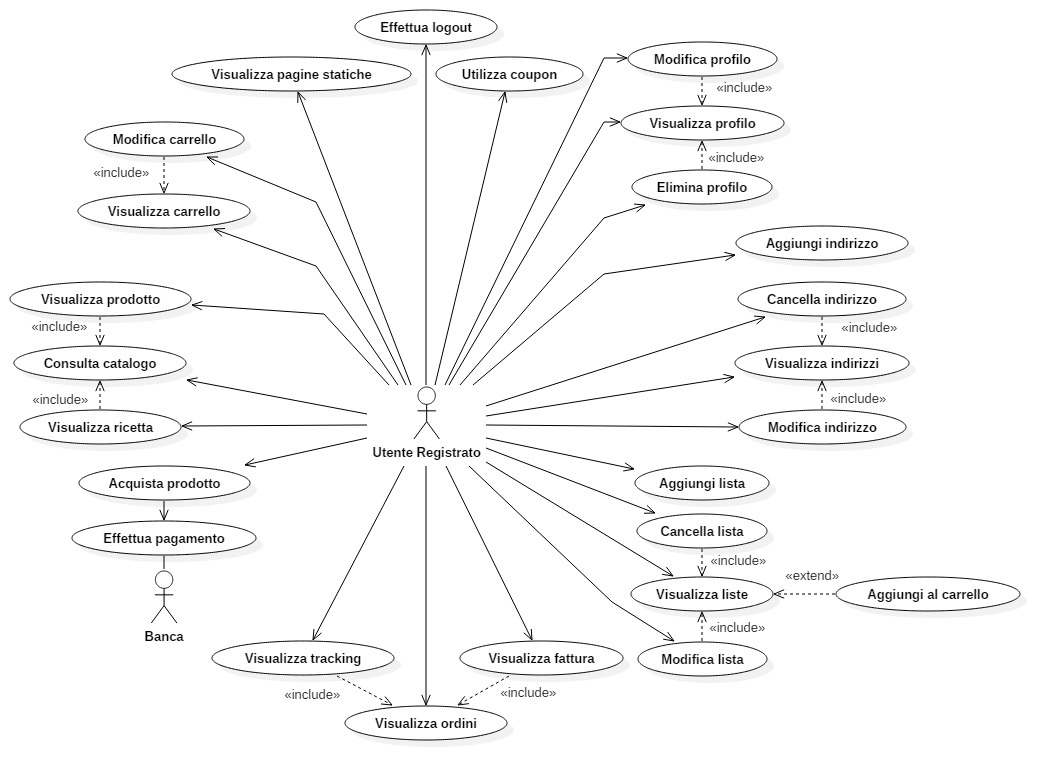
\includegraphics[width=1\textwidth]
	{immagini/attore-utente-registrato}
	
	\caption{Casi d'uso dell'attore utente registrato}
\end{figure}

\section{Attore utente super amministratore}
%
% Figura: casi d'uso dell'attore utente super amministratore
%
\begin{figure}[h]
	\centering
	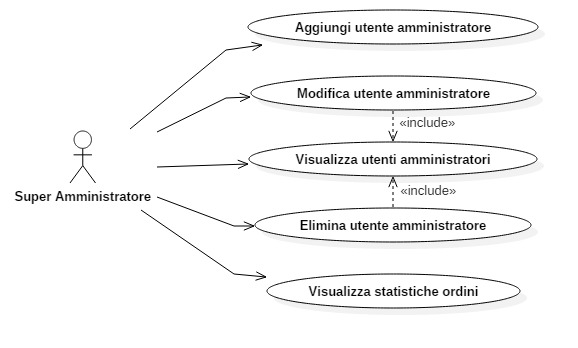
\includegraphics[width=1\textwidth]
	{immagini/attore-utente-super-amministratore}
	
	\caption{Casi d'uso dell'attore utente super amministratore}
\end{figure}

\section{Attore utente amministratore}
%
% Figura: casi d'uso dell'attore utente amministratore
%
\begin{figure}[h]
	\centering
	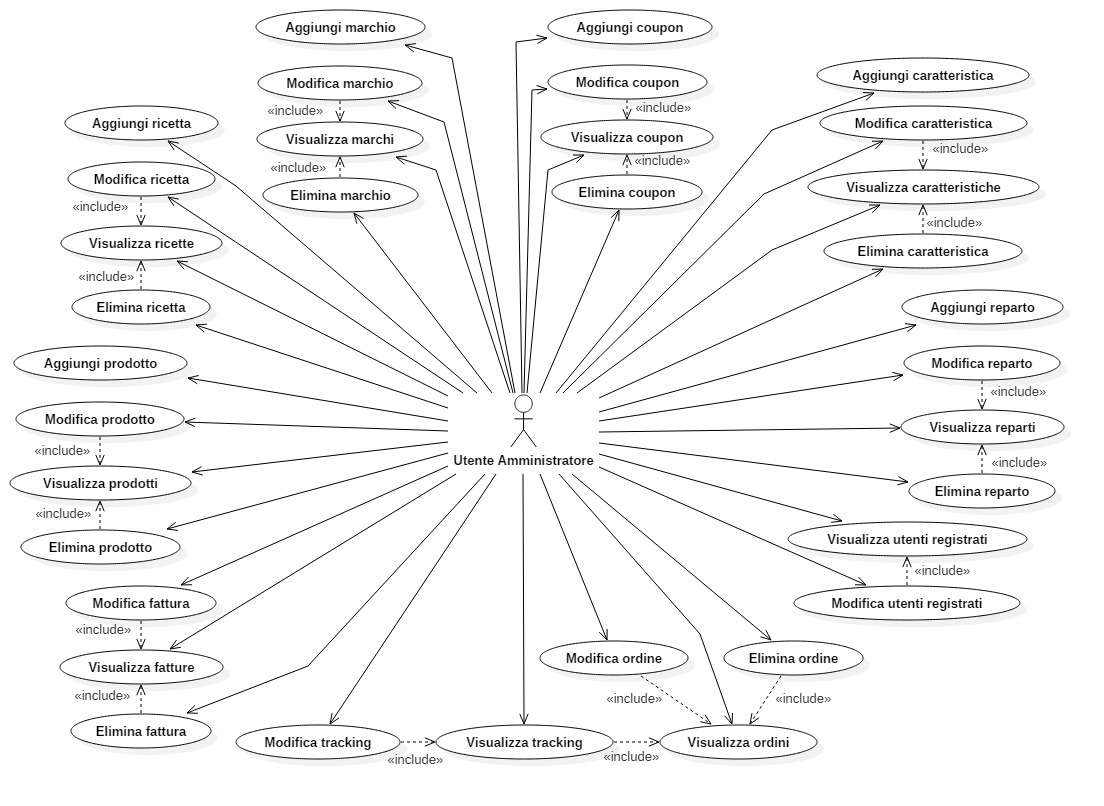
\includegraphics[width=1\textwidth]
	{immagini/attore-utente-amministratore}
	
	\caption{Casi d'uso dell'attore utente amministratore}
\end{figure}

\section{Diagramma delle attività}
\begin{enumerate}
	\item
	Consultazione catalogo
	
	\item
	Acquisto di un prodotto
	
\end{enumerate}   % modello dei casi d'uso
%\appendix
%\input{capitoli/Dolor}
% *****************************************************************
% Materiale finale
%******************************************************************
%% !TEX encoding = UTF-8
% !TEX TS-program = pdflatex
% !TEX root = ../Tesi.tex
% !TEX spellcheck = it-IT

%*******************************************************
% Bibliografia
%*******************************************************
\cleardoublepage
\nocite{*}
\printbibliography
%% !TEX encoding = UTF-8
% !TEX TS-program = pdflatex
% !TEX root = ../Tesi.tex
% !TEX spellcheck = it-IT

%*******************************************************
% Dichiarazione
%*******************************************************
\cleardoublepage
\phantomsection
\pdfbookmark{Dichiarazione}{Dichiarazione}
\chapter*{Dichiarazione}
\thispagestyle{empty}

Lorem ipsum dolor sit amet, consectetuer adipiscing elit. Ut purus elit, vestibulum ut, placerat ac, adipiscing vitae, felis. Curabitur dictum gravida mauris. Nam arcu libero, nonummy eget, consectetuer id, vulputate a, magna. Donec vehicula augue eu neque.

Pellentesque habitant morbi tristique senectus et netus et malesuada fames ac turpis egestas. Mauris ut leo. Cras viverra metus rhoncus sem. Nulla et lectus vestibulum urna fringilla ultrices.

\bigskip
 
\noindent\textit{\myLocation, \MakeTextLowercase{\myTime}}

\smallskip

\begin{flushright}
    \begin{tabular}{m{5cm}}
        \\ \hline
        \centering\myName \\
    \end{tabular}
\end{flushright}

\end{document}